\hypertarget{stm32f4xx__hal__uart_8c}{}\section{Dokumentacja pliku S\+T\+M/\+W\+D\+S\+\_\+\+Kosc\+\_\+\+Linux/\+Drivers/\+S\+T\+M32\+F4xx\+\_\+\+H\+A\+L\+\_\+\+Driver/\+Src/stm32f4xx\+\_\+hal\+\_\+uart.c}
\label{stm32f4xx__hal__uart_8c}\index{S\+T\+M/\+W\+D\+S\+\_\+\+Kosc\+\_\+\+Linux/\+Drivers/\+S\+T\+M32\+F4xx\+\_\+\+H\+A\+L\+\_\+\+Driver/\+Src/stm32f4xx\+\_\+hal\+\_\+uart.\+c@{S\+T\+M/\+W\+D\+S\+\_\+\+Kosc\+\_\+\+Linux/\+Drivers/\+S\+T\+M32\+F4xx\+\_\+\+H\+A\+L\+\_\+\+Driver/\+Src/stm32f4xx\+\_\+hal\+\_\+uart.\+c}}


U\+A\+RT H\+AL module driver. This file provides firmware functions to manage the following functionalities of the Universal Asynchronous Receiver Transmitter Peripheral (U\+A\+RT).  


{\ttfamily \#include \char`\"{}stm32f4xx\+\_\+hal.\+h\char`\"{}}\newline
Wykres zależności załączania dla stm32f4xx\+\_\+hal\+\_\+uart.\+c\+:\nopagebreak
\begin{figure}[H]
\begin{center}
\leavevmode
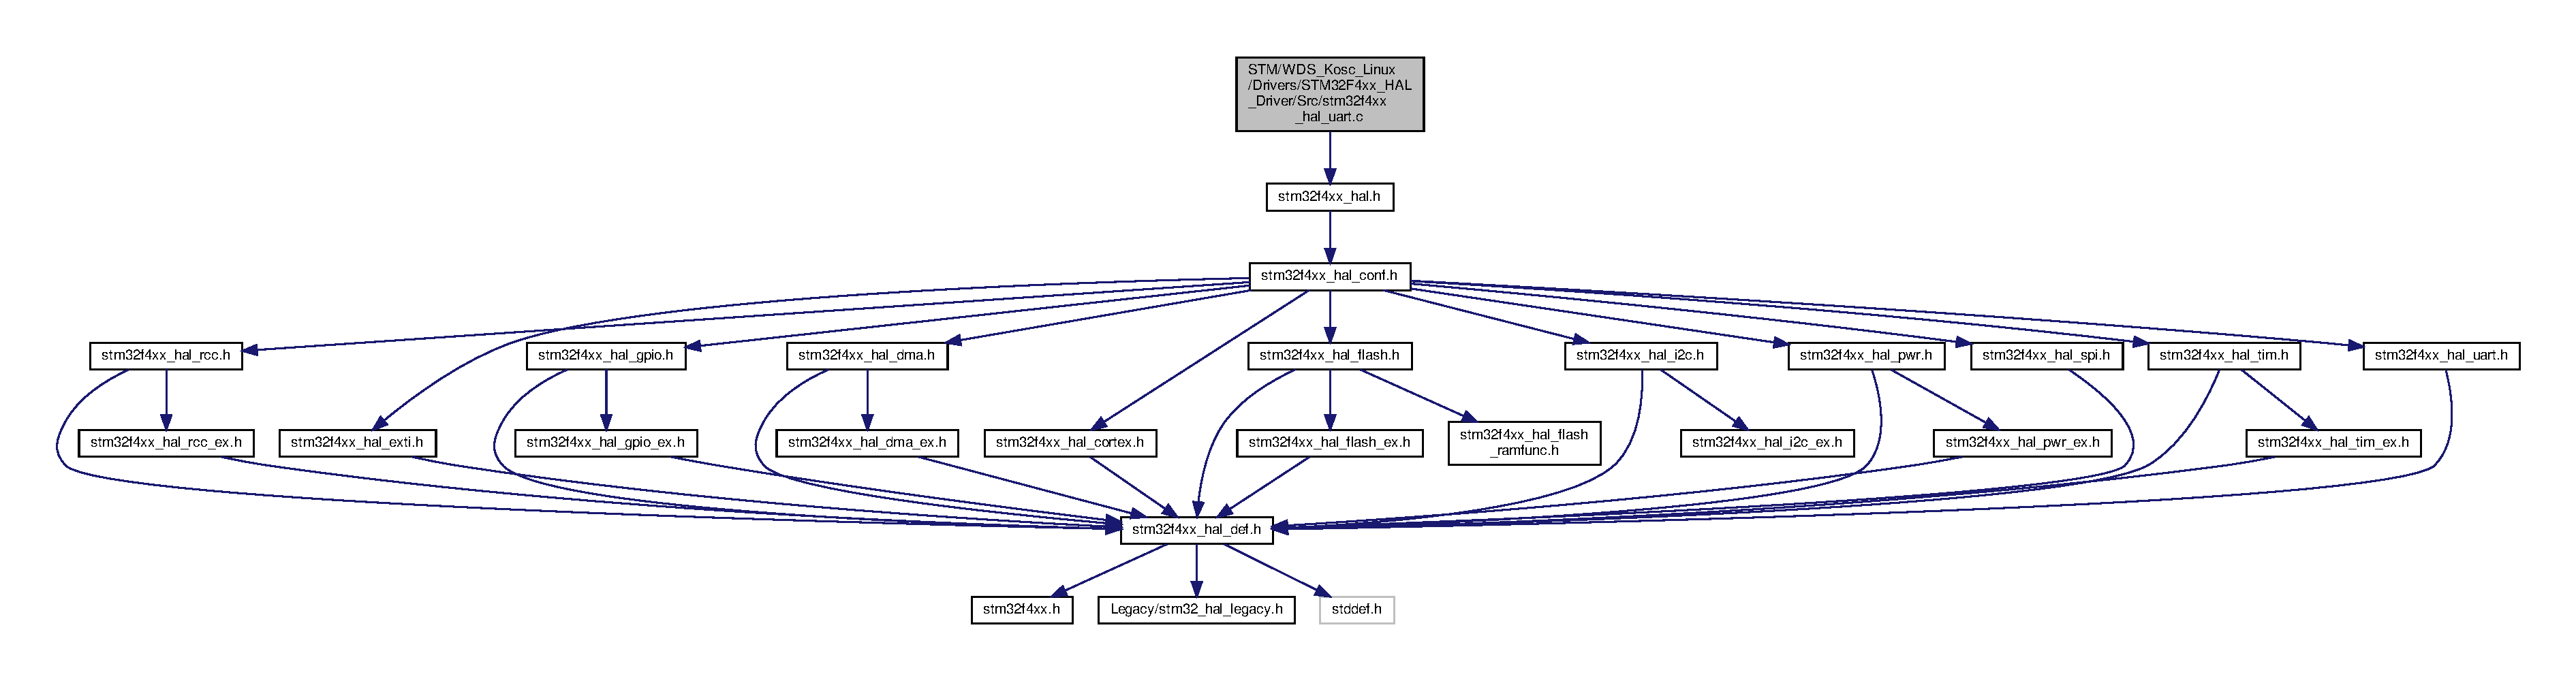
\includegraphics[width=350pt]{stm32f4xx__hal__uart_8c__incl}
\end{center}
\end{figure}


\subsection{Opis szczegółowy}
U\+A\+RT H\+AL module driver. This file provides firmware functions to manage the following functionalities of the Universal Asynchronous Receiver Transmitter Peripheral (U\+A\+RT). 

\begin{DoxyAuthor}{Autor}
M\+CD Application Team
\begin{DoxyItemize}
\item Initialization and de-\/initialization functions
\item IO operation functions
\item Peripheral Control functions
\item Peripheral State and Errors functions \begin{DoxyVerb}==============================================================================
                      ##### How to use this driver #####
==============================================================================
[..]
  The UART HAL driver can be used as follows:

  (#) Declare a UART_HandleTypeDef handle structure (eg. UART_HandleTypeDef huart).
  (#) Initialize the UART low level resources by implementing the HAL_UART_MspInit() API:
      (##) Enable the USARTx interface clock.
      (##) UART pins configuration:
          (+++) Enable the clock for the UART GPIOs.
          (+++) Configure these UART pins (TX as alternate function pull-up, RX as alternate function Input).
      (##) NVIC configuration if you need to use interrupt process (HAL_UART_Transmit_IT()
           and HAL_UART_Receive_IT() APIs):
          (+++) Configure the USARTx interrupt priority.
          (+++) Enable the NVIC USART IRQ handle.
      (##) DMA Configuration if you need to use DMA process (HAL_UART_Transmit_DMA()
           and HAL_UART_Receive_DMA() APIs):
          (+++) Declare a DMA handle structure for the Tx/Rx stream.
          (+++) Enable the DMAx interface clock.
          (+++) Configure the declared DMA handle structure with the required
                Tx/Rx parameters.
          (+++) Configure the DMA Tx/Rx stream.
          (+++) Associate the initialized DMA handle to the UART DMA Tx/Rx handle.
          (+++) Configure the priority and enable the NVIC for the transfer complete
                interrupt on the DMA Tx/Rx stream.
          (+++) Configure the USARTx interrupt priority and enable the NVIC USART IRQ handle
                (used for last byte sending completion detection in DMA non circular mode)

  (#) Program the Baud Rate, Word Length, Stop Bit, Parity, Hardware
      flow control and Mode(Receiver/Transmitter) in the huart Init structure.

  (#) For the UART asynchronous mode, initialize the UART registers by calling
      the HAL_UART_Init() API.

  (#) For the UART Half duplex mode, initialize the UART registers by calling
      the HAL_HalfDuplex_Init() API.

  (#) For the LIN mode, initialize the UART registers by calling the HAL_LIN_Init() API.

  (#) For the Multi-Processor mode, initialize the UART registers by calling
      the HAL_MultiProcessor_Init() API.

   [..]
     (@) The specific UART interrupts (Transmission complete interrupt,
          RXNE interrupt and Error Interrupts) will be managed using the macros
          __HAL_UART_ENABLE_IT() and __HAL_UART_DISABLE_IT() inside the transmit
          and receive process.

   [..]
     (@) These APIs (HAL_UART_Init() and HAL_HalfDuplex_Init()) configure also the
          low level Hardware GPIO, CLOCK, CORTEX...etc) by calling the customized
          HAL_UART_MspInit() API.

  ##### Callback registration #####
  ==================================

  [..]
  The compilation define USE_HAL_UART_REGISTER_CALLBACKS when set to 1
  allows the user to configure dynamically the driver callbacks.

  [..]
  Use Function @ref HAL_UART_RegisterCallback() to register a user callback.
  Function @ref HAL_UART_RegisterCallback() allows to register following callbacks:
  (+) TxHalfCpltCallback        : Tx Half Complete Callback.
  (+) TxCpltCallback            : Tx Complete Callback.
  (+) RxHalfCpltCallback        : Rx Half Complete Callback.
  (+) RxCpltCallback            : Rx Complete Callback.
  (+) ErrorCallback             : Error Callback.
  (+) AbortCpltCallback         : Abort Complete Callback.
  (+) AbortTransmitCpltCallback : Abort Transmit Complete Callback.
  (+) AbortReceiveCpltCallback  : Abort Receive Complete Callback.
  (+) MspInitCallback           : UART MspInit.
  (+) MspDeInitCallback         : UART MspDeInit.
  This function takes as parameters the HAL peripheral handle, the Callback ID
  and a pointer to the user callback function.

  [..]
  Use function @ref HAL_UART_UnRegisterCallback() to reset a callback to the default
  weak (surcharged) function.
  @ref HAL_UART_UnRegisterCallback() takes as parameters the HAL peripheral handle,
  and the Callback ID.
  This function allows to reset following callbacks:
  (+) TxHalfCpltCallback        : Tx Half Complete Callback.
  (+) TxCpltCallback            : Tx Complete Callback.
  (+) RxHalfCpltCallback        : Rx Half Complete Callback.
  (+) RxCpltCallback            : Rx Complete Callback.
  (+) ErrorCallback             : Error Callback.
  (+) AbortCpltCallback         : Abort Complete Callback.
  (+) AbortTransmitCpltCallback : Abort Transmit Complete Callback.
  (+) AbortReceiveCpltCallback  : Abort Receive Complete Callback.
  (+) MspInitCallback           : UART MspInit.
  (+) MspDeInitCallback         : UART MspDeInit.

  [..]
  By default, after the @ref HAL_UART_Init() and when the state is HAL_UART_STATE_RESET
  all callbacks are set to the corresponding weak (surcharged) functions:
  examples @ref HAL_UART_TxCpltCallback(), @ref HAL_UART_RxHalfCpltCallback().
  Exception done for MspInit and MspDeInit functions that are respectively
  reset to the legacy weak (surcharged) functions in the @ref HAL_UART_Init()
  and @ref HAL_UART_DeInit() only when these callbacks are null (not registered beforehand).
  If not, MspInit or MspDeInit are not null, the @ref HAL_UART_Init() and @ref HAL_UART_DeInit()
  keep and use the user MspInit/MspDeInit callbacks (registered beforehand).

  [..]
  Callbacks can be registered/unregistered in HAL_UART_STATE_READY state only.
  Exception done MspInit/MspDeInit that can be registered/unregistered
  in HAL_UART_STATE_READY or HAL_UART_STATE_RESET state, thus registered (user)
  MspInit/DeInit callbacks can be used during the Init/DeInit.
  In that case first register the MspInit/MspDeInit user callbacks
  using @ref HAL_UART_RegisterCallback() before calling @ref HAL_UART_DeInit()
  or @ref HAL_UART_Init() function.

  [..]
  When The compilation define USE_HAL_UART_REGISTER_CALLBACKS is set to 0 or
  not defined, the callback registration feature is not available
  and weak (surcharged) callbacks are used.

   [..]
      Three operation modes are available within this driver :

   *** Polling mode IO operation ***
   =================================
   [..]
     (+) Send an amount of data in blocking mode using HAL_UART_Transmit()
     (+) Receive an amount of data in blocking mode using HAL_UART_Receive()

   *** Interrupt mode IO operation ***
   ===================================
   [..]
     (+) Send an amount of data in non blocking mode using HAL_UART_Transmit_IT()
     (+) At transmission end of transfer HAL_UART_TxCpltCallback is executed and user can
          add his own code by customization of function pointer HAL_UART_TxCpltCallback
     (+) Receive an amount of data in non blocking mode using HAL_UART_Receive_IT()
     (+) At reception end of transfer HAL_UART_RxCpltCallback is executed and user can
          add his own code by customization of function pointer HAL_UART_RxCpltCallback
     (+) In case of transfer Error, HAL_UART_ErrorCallback() function is executed and user can
          add his own code by customization of function pointer HAL_UART_ErrorCallback

   *** DMA mode IO operation ***
   ==============================
   [..]
     (+) Send an amount of data in non blocking mode (DMA) using HAL_UART_Transmit_DMA()
     (+) At transmission end of half transfer HAL_UART_TxHalfCpltCallback is executed and user can
          add his own code by customization of function pointer HAL_UART_TxHalfCpltCallback
     (+) At transmission end of transfer HAL_UART_TxCpltCallback is executed and user can
          add his own code by customization of function pointer HAL_UART_TxCpltCallback
     (+) Receive an amount of data in non blocking mode (DMA) using HAL_UART_Receive_DMA()
     (+) At reception end of half transfer HAL_UART_RxHalfCpltCallback is executed and user can
          add his own code by customization of function pointer HAL_UART_RxHalfCpltCallback
     (+) At reception end of transfer HAL_UART_RxCpltCallback is executed and user can
          add his own code by customization of function pointer HAL_UART_RxCpltCallback
     (+) In case of transfer Error, HAL_UART_ErrorCallback() function is executed and user can
          add his own code by customization of function pointer HAL_UART_ErrorCallback
     (+) Pause the DMA Transfer using HAL_UART_DMAPause()
     (+) Resume the DMA Transfer using HAL_UART_DMAResume()
     (+) Stop the DMA Transfer using HAL_UART_DMAStop()

   *** UART HAL driver macros list ***
   =============================================
   [..]
     Below the list of most used macros in UART HAL driver.

    (+) __HAL_UART_ENABLE: Enable the UART peripheral
    (+) __HAL_UART_DISABLE: Disable the UART peripheral
    (+) __HAL_UART_GET_FLAG : Check whether the specified UART flag is set or not
    (+) __HAL_UART_CLEAR_FLAG : Clear the specified UART pending flag
    (+) __HAL_UART_ENABLE_IT: Enable the specified UART interrupt
    (+) __HAL_UART_DISABLE_IT: Disable the specified UART interrupt
    (+) __HAL_UART_GET_IT_SOURCE: Check whether the specified UART interrupt has occurred or not

   [..]
     (@) You can refer to the UART HAL driver header file for more useful macros\end{DoxyVerb}
 \mbox{[}..\mbox{]} (@) Additionnal remark\+: If the parity is enabled, then the M\+SB bit of the data written in the data register is transmitted but is changed by the parity bit. Depending on the frame length defined by the M bit (8-\/bits or 9-\/bits), the possible U\+A\+RT frame formats are as listed in the following table\+: +-\/-\/-\/-\/-\/-\/-\/-\/-\/-\/-\/-\/-\/-\/-\/-\/-\/-\/-\/-\/-\/-\/-\/-\/-\/-\/-\/-\/-\/-\/-\/-\/-\/-\/-\/-\/-\/-\/-\/-\/-\/-\/-\/-\/-\/-\/-\/-\/-\/-\/-\/-\/-\/-\/-\/-\/-\/-\/---+ $\vert$ M bit $\vert$ P\+CE bit $\vert$ U\+A\+RT frame $\vert$ $\vert$-\/-\/-\/-\/-\/-\/-\/-\/-\/-\/-\/-\/-\/-\/-\/-\/-\/-\/---$\vert$-\/-\/-\/-\/-\/-\/-\/-\/-\/-\/-\/-\/-\/-\/-\/-\/-\/-\/-\/-\/-\/-\/-\/-\/-\/-\/-\/-\/-\/-\/-\/-\/-\/-\/-\/-\/---$\vert$ $\vert$ 0 $\vert$ 0 $\vert$ $\vert$ SB $\vert$ 8 bit data $\vert$ S\+TB $\vert$ $\vert$ $\vert$-\/-\/-\/-\/-\/-\/---$\vert$-\/-\/-\/-\/-\/-\/-\/-\/---$\vert$-\/-\/-\/-\/-\/-\/-\/-\/-\/-\/-\/-\/-\/-\/-\/-\/-\/-\/-\/-\/-\/-\/-\/-\/-\/-\/-\/-\/-\/-\/-\/-\/-\/-\/-\/-\/---$\vert$ $\vert$ 0 $\vert$ 1 $\vert$ $\vert$ SB $\vert$ 7 bit data $\vert$ PB $\vert$ S\+TB $\vert$ $\vert$ $\vert$-\/-\/-\/-\/-\/-\/---$\vert$-\/-\/-\/-\/-\/-\/-\/-\/---$\vert$-\/-\/-\/-\/-\/-\/-\/-\/-\/-\/-\/-\/-\/-\/-\/-\/-\/-\/-\/-\/-\/-\/-\/-\/-\/-\/-\/-\/-\/-\/-\/-\/-\/-\/-\/-\/---$\vert$ $\vert$ 1 $\vert$ 0 $\vert$ $\vert$ SB $\vert$ 9 bit data $\vert$ S\+TB $\vert$ $\vert$ $\vert$-\/-\/-\/-\/-\/-\/---$\vert$-\/-\/-\/-\/-\/-\/-\/-\/---$\vert$-\/-\/-\/-\/-\/-\/-\/-\/-\/-\/-\/-\/-\/-\/-\/-\/-\/-\/-\/-\/-\/-\/-\/-\/-\/-\/-\/-\/-\/-\/-\/-\/-\/-\/-\/-\/---$\vert$ $\vert$ 1 $\vert$ 1 $\vert$ $\vert$ SB $\vert$ 8 bit data $\vert$ PB $\vert$ S\+TB $\vert$ $\vert$ +-\/-\/-\/-\/-\/-\/-\/-\/-\/-\/-\/-\/-\/-\/-\/-\/-\/-\/-\/-\/-\/-\/-\/-\/-\/-\/-\/-\/-\/-\/-\/-\/-\/-\/-\/-\/-\/-\/-\/-\/-\/-\/-\/-\/-\/-\/-\/-\/-\/-\/-\/-\/-\/-\/-\/-\/-\/-\/---+
\end{DoxyItemize}
\end{DoxyAuthor}
\begin{DoxyAttention}{Uwaga}

\end{DoxyAttention}
\subsubsection*{\begin{center}\copyright{} Copyright (c) 2016 S\+T\+Microelectronics. All rights reserved.\end{center} }

This software component is licensed by ST under B\+SD 3-\/\+Clause license, the \char`\"{}\+License\char`\"{}; You may not use this file except in compliance with the License. You may obtain a copy of the License at\+: opensource.\+org/licenses/\+B\+S\+D-\/3-\/\+Clause 